\documentclass{article}
\title{Twiddle -- A DSL for the Functional Bit-hacker}
\author{Michael Buch}

\usepackage[inline]{enumitem} % inline numbered lists
\usepackage[left=2cm,right=2cm]{geometry}
\usepackage{verbatim} % for comments
\usepackage{graphicx}
\usepackage{listings}
\usepackage{color}
\usepackage{flafter}

\raggedbottom

\definecolor{dkgreen}{rgb}{0,0.6,0}
\definecolor{gray}{rgb}{0.5,0.5,0.5}
\definecolor{mauve}{rgb}{0.58,0,0.82}
\lstset{frame=tb,
  aboveskip=3mm,
  belowskip=3mm,
  showstringspaces=false,
  columns=flexible,
  basicstyle={\small\ttfamily},
  numbers=none,
  numberstyle=\tiny\color{gray},
  keywordstyle=\color{blue},
  commentstyle=\color{dkgreen},
  stringstyle=\color{mauve},
  breaklines=true,
  breakatwhitespace=true,
  tabsize=3
}

\begin{document}
\maketitle
\frenchspacing

\begin{abstract}
It is useful (and fun!) to bit twiddle i.e. perform arithmetic and manipulate data at the granularity of individual bits. Traditionally there is a compromise one has to make between using a low-level unsafe language that allows bit-twiddling versus a safe high-level language in which the type system or language design prohibit operations at bit-level (without additional complexity). The \textit{Twiddle} domain-specific language (DSL) is an embedded language written in Scala that generates bit-twiddling style C code. The language offers several modes of operation, useful for quick prototyping, debugging and custom extensions:
\begin{enumerate*}[label=(\arabic*)]
	\item Tracing interpreter
	\item Scala evaluator
	\item Twiddle AST generator
	\item C code generator
\end{enumerate*}.
Thus our language is a tool for the curious, a tool for safe bit-hackers and a tool for someone looking to get a bit more performance out of his high-level language.
\end{abstract}

\section{Motivation}
Bit-twiddling offers performance, especially when inquiring about or operating on the bit pattern itself. However, reasoning about the final code is a daunting task and despite the fun-factor utility it can provide, programmers actually requiring to use such an algorithm would benefit from a verified solution built-into their language. The need for bit-twiddling most commonly arises in applications that actually care about the binary representation of an integer such as error-correction schemes. A programmer in such a situation essentially has two choices:
\begin{enumerate*}[label=(\arabic*)]
	\item write an application in a low-level language like C and implement the readily available bit-hacks in it
	\item use a higher level language and accept the overheads it incurs
\end{enumerate*}. This project proposes an alternative in which we code-generate low-level code from a safer high-level language meanwhile preserving bit-twiddling operations. We embed a miniature interpreted language within Scala, that permits evaluation but also code generation of C code. Thus a programmer can focus on the problem rather than the implementation details. One benefits from Scala's type-system and the the object language's expressiveness and pointer-freeness while being able to generate generate bithacks. Additionally, a user of said generated code can be reassured that the semantics of the bithacks implemented in the ``Twiddle'' language have been verified by the authors \cite{anderson2005bit}. However, verifying the actual generated Twiddle code is not yet supported but could be realized in a similar fashion to Amin et al.'s generative verification framework \cite{amin2017lms}.

\pagebreak
\subsection{Example}
We start with a simple snippet from the user-level language, a mixture between Scala (the variable assignment) and a simple-term language (the if-then construct):
\begin{lstlisting}[language=Scala]
def snippet[T[_]](s:Exp[T]) = {
    import s._
    val a = bits(num(20))
    (ifThen(hasZero(a))
            (() => swapBits(a, bits(log10(num(30))))))
}
\end{lstlisting}
The type parameter \texttt{T[\_]} represents the type wrapper that the evaluator \texttt{s: Exp[T]} uses to wraps its abstract type. We invoke the snippet as follows:
\begin{lstlisting}[language=Scala]
val evaluated = snippet(Eval)
val ast = snippet(EmitTwiddleAST)
\end{lstlisting}
Here we see the interpretation of the same snippet in two wildly different forms. The first line evaluates directly and yields the swapped bits using Scala's \texttt{BitSet} type:
\begin{verbatim}
    (BitSet(0),BitSet(2, 4))
\end{verbatim}
The second line, however, emits the AST using the \texttt{EmitTwiddlAST} evaluator, yielding:
\begin{verbatim}
    Tup(Decl(I(Var(cond3))),
        Tup(Decl(U(Var(cons4))),
            Tup(Assign(Var(cond3),
                Result(Var(r2) <--- snipped -->
\end{verbatim}

When we pass the AST output to the code generator, i.e. \texttt{Codegen.gensrc(snippet(EmitTwiddleAST))} we get the following C code (with stylistic modifications):

\begin{lstlisting}[language=C]
// <--- Snipped --->
#define HAS_ZERO(v) (((v) - 0x01010101UL) & ~(v) & 0x80808080UL)
#define SWAP(a, b) (((a) ^= (b)), ((b) ^= (a)), ((a) ^= (b)))
int main() {

	int cond35;
	unsigned int cons36;
	unsigned int r34;
	unsigned int v33;
	v33 = 20;
	r34 = HAS_ZERO(v33);
	cond35 = r34;

	if(cond35) {
		unsigned int r40;
		unsigned int v38;
		unsigned int v39;
		v38 = 20;
		int ret37;
		ret37 = (30.0 >= 1000000000) ? 9 : (30.0 >= 100000000) ? 8 : (30.0 >= 10000000) ? 7 : (30.0 >= 1000000) ? 6 : (30.0 >= 100000) ? 5 : (30.0 >= 10000) ? 4 : (30.0 >= 1000) ? 3 : (30.0 >= 100) ? 2 : (30.0 >= 10) ? 1 : 0;
		v39 = ret37;
		r40 = SWAP(v38,v39);
		cons36 = r40;
	}

	return 0;
}
// END OF CODE GENERATED BY TWIDDLE
\end{lstlisting}

This demonstrates our goal of producing bit-twiddled code from a safer high-level language without have to worry about syntax, details of bit representation, operator precedence or undefined behaviour. In the example  the resulting value can be retrieved from variable \texttt{cons36}.

\section{Run Instructions}
\subsection{Running Tests}
The project structure is adapted to the Scala ``sbt'' build tool. The \textbf{src/main/twiddle-tests.scala} contains feature test cases that showcase some of the functionality of Twiddle. To run them simply
run \texttt{sbt run} from the the root directory.

\subsection{Creating Snippets}
\begin{enumerate}
	\item Create a new file or use \textbf{src/main/playground.scala}
	\item Create a function with following structure:
	\begin{verbatim}
		def example[T[_]](s:Exp[T]) = {
		    import s._
		    // Twiddle code goes here...
		}
	\end{verbatim}
	\item Then call the function e.g. from a main() function, using one of the supported evaluators. When using \texttt{EmitTwiddleAST} you have several options of how to treat the AST currently:
	\begin{itemize}
		\item \texttt{Codegen.eval(example(EmitTwiddlAST))}
		\item \texttt{Codegen.gensrc(example(EmitTwiddlAST))}
		\item \texttt{Codegen.runsrc(Codegen.gensrc(example(EmitTwiddlAST)))}
	\end{itemize}
	The first will simply emit the Twiddled C code to stdout. The second method will generate a file called	\textbf{twiddle.c} that contains the emittted source. The third option shows how to run the emitted source. \texttt{Codegen.runsrc(...)} will compile and run \textbf{twiddle.c}.
	\item Run from the root directory: sbt run
\end{enumerate}

\section{The Language \& Architecture}
\begin{figure}[t]
	\centering
	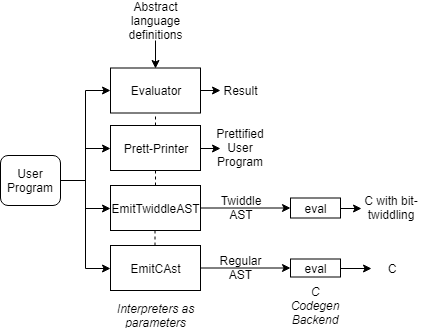
\includegraphics[scale=0.8]{twiddle_arch.png}
	\caption{Architecture of the Twiddle framework}\label{twiddle_arch}
\end{figure}
\subsection{Core}
The core of the language is split into modular pieces of functionality implemented as traits. As is common practice with tagless final interpreters (see section \ref{subsec:tagless}) we create an abstract type \texttt{Exp[T[\_]]} parameterized by an evaluator. Each set of language features is then implemented as a function in an evaluator that describes the feature's behaviour in the evaluator's context. Simply said, we turn terms in the host language into functions in the object language. We bundle similar language features into a set of traits. Some of these features (defined \textbf{core.scala}) are described below:
\begin{itemize}
	\item \textbf{Nums}: Defines abstract interpretation of numeric Scala types including \texttt{Int, Double, Float}. It is generic over the type of input number supplied. Operations involving numeric types in the core language thus have to also be generic over numeric types. This is fine for integral numbers but gets problematic for fractional operations such as division.
	\item \textbf{Arithmetic}: Basic mathematical operations that operate on the interpretation of core's \texttt{num}. Some operations are generic over the input type while others are explicitly for fractional versus integral types.
	\item \textbf{Bools}: Includes both the interpretation of Scala's \texttt{Boolean} type and also of constructs operating on said booleans such as if-statements, ternary operators and logical operators.
	\item \textbf{Lambda}: Interpretation of lambda definition and application. Scala's lambda maps cleanly to the concept of a lambda in the lisp-like user-level language. However, a mapping to C is less straightforward and described in section \ref{subsec:ast_interpreter}
	\item \textbf{LispLike}: Contains a limited set of Lisp primitives to be able to create lists using \texttt{cons/car/cdr}. A \texttt{begin} primitive was added mainly as a way to collect the AST nodes created in a code snippet when interpreting using \texttt{EmitTwiddleAST} since without it Scala would simply return the last generated statement. Essentially it is a wrapper around a Scala \texttt{List}.
\end{itemize}

The traits prefixed with a ``C'' such as the following ones listed are the operations taken from Anderson's set of bithacks\cite{anderson2005bit}.
\begin{itemize}
	\item \textbf{CMathOps}: Mathematical operations that when passed to the codegeneration backend produce bit-twiddled implementations. Typically in other languages these would correspond to standard library functions such as \textbf{scala.math.log10} for \texttt{log10}.
	\item \textbf{Bits}: Includes definitions of the \texttt{bits} term, which is simply the interpretation of a numeric type, and functions whose goal is to operate on the structure of bit patterns of an integer such as reversing bit sequences.
\end{itemize}

\subsection{Evaluators}
Each term in the language is a function whose parameters and return type are wrapped in the abstract type of the interpreter that is evaluating the function. The second column of figure \ref{twiddle_arch} shows the current set of supported interpreters.

\textit{Evaluator} corresponds to the \texttt{implicit object Eval} in \textbf{interpreter.scala}. Here terms are evaluated and returned as values in the host language (i.e. Scala).

\textit{Pretty-Printer} corresponds to the \texttt{implicit object Show} in \textbf{interpreter.scala}. Here all terms are of type \texttt{String} and evaluation of a term yields its pretty-printed version.

\textit{EmitTwiddleAST} corresponds to the Scala object of the same name in \textbf{ast-interpreter.scala}. This is the core of the Twiddle code generator.

\textit{EmitParallelAST} corresponds to the \texttt{implicit object EmitParallelAST} in \textbf{ast-interpreter.scala}. This evaluator produces an AST with annotations for parallelization. The code generator uses the annotations to generate additional OpenMP pragmas.

\section{Codegen}
\subsection{Twiddle AST}
The code generation part of the Twiddle framework is shown in the bottom two branches of the flow chart in figure \ref{twiddle_arch}. As a way to map modularly and extensibly between a high-level language like the lambda calculus variant in our case to a low-level language like C we introduced a intermediate representation (IR) of the user-level Twiddle code structured as an abstract syntax tree (AST). The IR language includes features that would not fit to the semantics of the high-level language but are needed for bit-twiddling or general operations in C. Nodes in the AST are all represented by the \texttt{abstract trait Term} and evaluation of the terms occurs on nested tuples of terms (i.e. \texttt{Tup(Term, Tup(Tup(Term, Term)...)...)}) to be able to conveniently manipulate it from within the evaluator of the AST. Where there is only a small set of one-to-one mappings between terms in the object language and actual C language constructs, the IR mimics a subset of valid terms in C. Figure DIAGRAM NEEDED shows valid terms in the Twiddle IR. Distinction between primitives, expressions, C language identifiers, etc. is not provided since our evaluators on the AST did not require it. The term types can, however, be refined with additional traits if one needs to special-case according to certain classes of C language features.

\subsubsection{Builtins}
There is no distinction between language features and built-in functions in Twiddle. Every language feature is a function that describes its evaluation in the interpreter context. We implement common operations in the associated traits and inject it into the abstract \texttt{Exp[T[\_]]} trait. These operations have been chosen with bit-twiddling in mind. More often than not there is a corresponding algorithm using bithacks \cite{anderson2005bit} which the codegen back-end implements in the IR.

We considered several ways of supporting bit-twiddling operations. In the final version of Twiddle we have a specific bit-twiddling backend whose sole purpose is to translate arithmetic, string or bit operations, provided as language features, into equivalent bithacks. While a step in the right direction, an alternative (or extension) would be to detect certain user patterns or even annotations in the source, and map the patterns into bithack patterns. An example could be the reversal of a string. If currently a user is not aware of the Twiddle provided builtin \texttt{reverse(s: T[String])}, a user might choose to implement his own reversal algorithm and Twiddle would simply generate plain C. A more advanced backend detects these patterns from the AST.

\subsubsection{Bits}
So far we have only discussed mathematical or string operations that utilize arithmetic or logical shift operators to achieve a task that would have required control flow constructs in a naive implementation. The term bit-twiddling, however, also encompasses operations directly on the bit representation of terms. For this purpose, we implemented the \texttt{bits(a: T[Int]): T[BitSet])} term in the core language. As the function definition implies, an evaluation of \texttt{bits} will turn an integer into a logical representation of bits. We say logical representation because this translation is different between the Twiddle front-end evaluators and the codegen IR. In the Twiddle AST bits are simply represented as integers. Operations on said integers that would in the C layer operate on bits are responsible for declaring the necessary integers as \texttt{unsigned long}. In the front-end evaluator, however, a conversion does take place from integer to a Scala BitSet.

\subsubsection{Other Useful Constructs}
As implied above, not all IR terms are features in the core language, thus terms such as \texttt{Ref(e: Term)} or \texttt{Assign(v: Term, e: Term)} are helper terms used to ease the transition from user-level language to C.
Variable declarations and assignment

\subsection{Twiddle AST Interpreters}\label{subsec:ast_interpreter}
A consequence of the Tagless style of the core language is that in order to achieve a generic expression type that is used across all interpreters and be able to interpret the same piece of code in multiple ways, we need to implement language features across several interpreters that are semantically sound. For the \texttt{EmitTwiddleAST} interpreter this poses a challenge since some of the functional higher-level constructs do not map cleanly onto C-style programs. A prime example is the lambda/apply pair. A way to map lambdas to C is to convert the lambda into a function definition, storing the function body together with a unique function name in the internal interpreter state, return the function name to the user and on applications of the function name generate a C function call. For this purpose we implemented term \texttt{Func( FILL )} and \texttt{App( FILL )}. However, retrieving the function body requires intrusive changes around several components of the framework and is left as an open exercise for future versions. Currently a \texttt{lam} returns a closure to the user which he is responsible for applying i.e. passing to \texttt{app} which then evaluates the lambda.

\subsubsection{Auxiliary Machinery}
To avoid name clashes we use a file-static counter that increments whenever a call to \texttt{gensym} is performed.

In procedural languages one has to be able to assign an expression to a variable to track state and perform any kind of meaningful computation. This is problematic in our ``greedy-print'' model of code generation since we can generate syntactically invalid expression assignments. An example would be generating code from:
\begin{lstlisting}[language=Scala]
val x = 5
val y = add10(x)
val z = 2 * y
\end{lstlisting}
\begin{lstlisting}[language=C]
int z = 2 * int x = 5; + 10 // Syntax error
\end{lstlisting} Since we do not perform constant propagation or evaluation of terms prior to emitting Twiddle source, we need a mechanism to signal that an expression returns a meaningful result and a subsequent expression should use that value instead. Taking inspiration from Let-insertion in ANF-conversion of functional languages, we introduced a \texttt{Result(v: Var, t: Term)} into the IR that will assign the result of evaluating some expression $t$ to the variable $v$ in the generated code.

%To overcome some of Scala's type parameter constraints without adding unnecessary complexity, we introduce a dependency on the \textit{shapeless} framework \footnote{https://github.com/milessabin/shapeless} which permits casting on type parameters even in the presence of type erasure. The main use is the casting of numeric types to a Scala \texttt{Long} when passing them to the \texttt{bits} evaluation.

To make sure the C preprocessor directives such as \texttt{\#include} and \texttt{\#define} are kept at the top of the file (although generally speaking C programmers might not want this), we keep a file global list of defines together with metainformation about them, such as name, paramters and body. We collect the information during AST evaluation and emit them
during code generation (in \texttt{Codegen.gensrc(...)}).
\section{Design Choices}
\subsection{Scala}
We chose Scala for primarily for following reasons:
\begin{itemize}
	\item Functional features that benefit implementation complexity
	\item Flexible type sytem
	\item Reflection capabilities
	\item Library support for staging
\end{itemize}

The combination of Scala ability to create type classes, pattern matching, first-class functions and mature reflection capabilities are a well-suited foundation
for writing an interpreter or embed a DSL into it. We make use of type classes \cite{wadler1989make} to implement our tagless interpreter by having traits that represent
the DSL's language features be defined for multiple implementations. Where we face issues with implementing functionality for individual interpreters, for example due to restrictions imposed by
that interpreters abstract type (or sub-optimal design decisions), we use reflection in the form of \texttt{ClassTag} or \texttt{TypeTag}. Our code generation backend is essentially a
pattern matcher on terms.

The last point in regards to Rompf et al.'s Leightweight Modular Staging framework \cite{rompf2010lightweight} that uses type-driven staging to perform automatic binding time analysis and
program specialization. It is attractive due to its extensibility to ones own DSL, providing multiple code generation targets including C and CUDA, which would have been ideal for Twiddle. Unfortunately, practical
limitations including the lack of flexibility to implement control the amount, name and properties of generated variables (without significant implementation overhead). Additionally, because LMS shares code generation
facilities between C++ and C, finding the correct combination of traits to mix into the Twiddle DSL to generate \textit{standard} C without creeping C++ into the mix proved challenging. After initial implementaiton using LMS
we instead dropped support for the framework and instead built our own code generation facilities. However, since other DSLs targeting C have been implemented using LMS successfully \cite{lee2011implementing, amin2017lms}, a future iteration of Twiddle could have its
code generation and optimization be done through LMS.

Of course similar features are avaiable in languages like Haskell and Ocaml and stagin/metaprogramming facilities in frameworks like Template Haskell and MetaOcaml, however, due to experience with prior Scala and its mature and a reflection API that is part of the \textit{language standard}
served as an advantage over the alternatives.

\subsection{Partially Tagless Final Style Embeddings}\label{subsec:tagless}
EXPLAIN TAGLESS STYLE USING PAPER While the core language is implemented as a tagless-final interpreter, our code generation backened uses a tagged approach. An advantage of a tagless approach is that encourages to carefully think about the type signatures of the core language features. Since a term's interpretation
can vastly differ between evaluators depending on the choice of abstract type wrapper, a poorly chosen API can lead to difficult implementations that work across all evaluation schemes and can potentially cause the implementor to tap into a host language's reflection capabilities.

An alternative to our case-based code generation could have been to implement the code generation as just another tagless interpreter and skip the creation of an AST. However, this could prove cumbersome to combine with optimization passes such as a parallelizer that works best on a graph based representation of a program. Ultimately,
the pipeline remains the same: First build an IR of the program. Then transform the IR into target.

Since C is a language of vastly different structure and semantics than both the host language and the user-level language, a separation between front-end evaluation and code-generation could benefit the extensibility of the framework. Essentially we can now imagine alternative AST generators, ones that produce an AST with nodes that are optimized for example w.r.t code size instead of just being twiddled. Our design achieves
a clear separation between analysis of the object language and the act of mere code-generation which can be reused for multiple forms of the AST.

One downside of our approach is that we basically have to model the entire C language's semantics in our AST to be practical.

NOTE: the dsl AST evaluator could be a tagless interpreter itself => instead of having AST node terms implement them as function definitions over abstract types

\subsection{Lessons Learned}
TODO
Value of tagless final
alternative methods of emitting C->should probably follow semantics of the codegenned language

\begin{itemize}
	\item Benefits of shallow embeddings. Can fall back to scala features. Don't need to implement side effects in object language necessarily.
	\item Extend LMS
	\item Use tagless evaluator for AST evaluation
	\item Writing larger programs
	\item Other backends
	\item Staging
	\item Parallelizing backend -> would be better suited as an evaluator on the AST
	\item eliminate need for redundant reassignments (reference example)
	\item Instead of mapping from DSL to tiwddled C immediately could first map to C and then optionally bit-twiddle
\end{itemize}

tagless if one interprets in vastly different manners for different use cases it can get difficult to choreograph the types to work properly although Scala helps with its type inference and type system flexibility
\section{Conclusion \& Future Work}
Current limits of the framework include the amount of supported language features, intersection of the supported types between the user-language and C and the number of evaluators avaiable. Additionally, much of the current DSL fits the structure
that the Scala LMS framework expects to be able to add code-generation and optimization facilities to multiple backends.

Our language currently only supports basic string, integer and 32-bit bit types. C additionally supports various numeric unsigned/signed/numeric/fractional types of different sizes. Moreoever, we do not not support collection types such as arrays or structs (although they can be emitted through pointers via the AST). A natural improvement to Twiddle would be the extension of the core language
to a larger conformance with the C language.

A useful additional extension could be the verification of the output language. For this one could add annotations to the code that conform with available C verification backends such as Frama-C. Another option would be to investigate extensions to existing verified-C generation frameworks such as ``lms-verify'' \cite{amin2017lms}.

\bibliographystyle{ieeetran}
\bibliography{twiddle}
\end{document}
